\documentclass{beamer}
\usepackage[utf8]{inputenc}
\usepackage{graphicx}
% TEMA DE LA PRESENTACIÓN
\usetheme{split}
\useinnertheme{circles}
\usepackage{beamerthemeshadow}
% COLOR DE LA PÁGINA
\usestructuretemplate{\color{structure}}{}
\beamertemplateshadingbackground{yellow!50}{blue!50}
% DATOS DE PRESENTACIÓN
\title{El software libre en la vida diaría}
\subtitle{FLISoL 2020} 
\author{José Vidal Cardona Rosas}
\institute{ENES, Morelia Mich.} 
\begin{document}
    % Frame DATOS DE PRESENTACIÓN
    \begin{frame}
        \titlepage
    \end{frame}

    % Frame ESQUEMA DE LA PLÁTICA
    \section{Esquema de la plática}
    \begin{frame}
        \frametitle{Esquema de la plática}
        %\tableofcontents[currentsection]
        \begin{block}{Temas a conocer}
            \begin{itemize}
                \item \textbf{¿Qué es el Software Libre?}
                \begin{itemize}
                    \item \textbf{¿Y el Open Source?}
                \end{itemize}
                \item \textbf{Diferencias entre Software Libre 
                y Open Source}
                \begin{itemize}
                    \item \textbf{¿Qué objetivos persiguen?}
                \end{itemize}
                \item \textbf{Software Libre de uso diario}
                \item \textbf{¿Cómo me beneficia el uso de
                Software Libre?}
                \item \textbf{Limitantes del Software Libre
                frente al Software de paga}
                \item \textbf{Dando el salto: Pasando de ser
                consumidor a creador}
            \end{itemize}
        \end{block}
    \end{frame}

    % Frame ¿QUÉ ES EL SOFTWARE LIBRE?
    \section{¿Qué es el software libre?}
    \begin{frame}
     \frametitle{¿Qué es el software libre?}
     \framesubtitle{¿Y el Open Source?}
     \textbf{Software libre:} Es el software que respeta las libertades de los usuarios y de la 
     comunidad.
     \begin{figure}[b]
     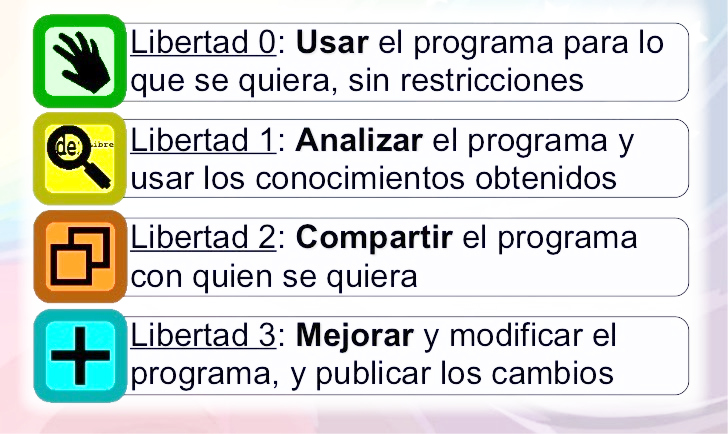
\includegraphics[scale=1]{libertades(1).jpg}
      \centering
     \end{figure}
     
     
    \end{frame}
    % Frame SOFTWARE LIBRE Y OPEN SOURCE
    \section{Software Libre Y Open Source}
    \begin{frame}
        \frametitle{Diferencias entre Software Libre y Open Source}
      
        
        El \textbf{\textit{Software Libre}}: 
        \begin{itemize}
            \item Más radical
            %\item Inmutable
            \item El usuario puede hacer con el código lo que sea, pero sin 
            cambiar la licencia o venderlo
        \end{itemize}
        
        El \textbf{\textit{Open Source}}:
        \begin{itemize}
         \item Menos radical
         \item Ofrece opciones al usuario final (con y sin fines de lucro)
        \end{itemize}
        \footnote{La gran diferencia entre Software Libre y Open Source: https://www.gnu.org/philosophy/open-source-misses-the-point.html}
    \end{frame}

    % Frame SOFTWARE LIBRE DE USO DIARIO
    \section{Software libre de uso diario}
    \begin{frame}
        \frametitle{Software libre de uso diario}
        
\includegraphics[scale=0.25]{BeFunky-collage.jpg}
        \centering
    \end{frame}
    % Frame ¿CÓMO NOS BENEFICIA EL SOFTWARE LIBRE?
    \section{¿Cómo me beneficia el Software Libre?}
    \begin{frame}
     \frametitle{¿Cómo me beneficia el Software Libre?}
     ''La palabra \textbf{free} tiene dos significados. Puede referirse a la libertad o al precio. Cuando hablamos de software libre (free software), estamos hablando de libertad, no de precio.''\\
     (Free Software Foundation 2020)
     \begin{figure}[h]
     \includegraphics[scale=0.4]{SDollar.jpg}
      \centering
     \end{figure}
     \footnote{Vender software libre: https://www.gnu.org/philosophy/selling.html}
    \end{frame}

    % Frame LIMITANTES DEL SOFTWARE LIBRE FRENTE AL DE PAGA
    \section{Limitantes del Software Libre frente al de paga}
    \begin{frame}
     \frametitle{Limitantes del Software Libre frente al de paga}
     \begin{itemize}
        \item Ausencia de garantía
        \item Baja difusión
        \item Diversidad de distribuciones
        \item La curva de aprendizaje es mayor que en el de paga
     \end{itemize}

    \end{frame}

    % Frame DANDO EL SALTO: PASANDO DE SER CONSUMIDOR A SER CREADOR
    \section{Dando el salto: Pasando de ser consumidor a ser creador}
    \begin{frame}
     \frametitle{Dando el salto: Pasando de ser consumidor a ser creador}
     % Botón de play para vídeo
     \beamergotobutton{Vídeo}
    \end{frame}
    
    \section{Información de contacto}
    \begin{frame}
    \frametitle{Información de contacto}
     \begin{figure}[h]
     
\includegraphics[scale=0.2]{redes.jpg}
      \centering
     \end{figure}
    \end{frame}
    
    \begin{frame}
     \frametitle{Referencias}

       \tiny{* Ing. Gina E. Valencia Mendoza, G. E. (s.f.). VENTAJAS Y DESVENTAJAS DEL SOFTWARE LIBRE [Publicación en un blog]. Recuperado 23 marzo, 2020, de http://andreitamedina.blogspot.com/2012/04/ventajas-y-desventajas-del-software.html}\newline
      
       \tiny{* Selling Free Software - GNU Project - Free Software Foundation [Publicación en un blog]. (s.f.). Recuperado 23 marzo, 2020, de https://www.gnu.org/philosophy/selling.html}\newline
      
       \tiny{* SDPnoticias.com. (2012, 30 abril). "Desventajas" del Software Libre [Publicación en un blog]. Recuperado 23 marzo, 2020, de https://www.sdpnoticias.com/columnas/desventajas-software-libre.html}\newline
      
       \tiny{* 10 Ejemplos de Software Libre [Publicación en un blog]. (s.f.). Recuperado 23 marzo, 2020, de https://10ejemplos.com/10-ejemplos-de-software-libre/}\newline
      
       \tiny{* Flores, M. flores. (2020, 11 febrero). Ejemplos de Software Libre [Publicación en un blog]. Recuperado 23 marzo, 2020, de https://www.elmundogeek.com.mx/tecnologia/ejemplos-de-software-libre/}\newline
      
       \tiny{* ¿Qué es el software libre? - Proyecto GNU - Free Software Foundation [Publicación en un blog]. (s.f.). Recuperado 23 marzo, 2020, de https://www.gnu.org/philosophy/free-sw.es.html}

    \end{frame}

    


    

\end{document}
